\documentclass[border=8pt]{standalone}
\usepackage{fontspec}
\setmainfont{TeX Gyre Heros}[Ligatures=TeXOff]
\XeTeXgenerateactualtext=1
\setsansfont{TeX Gyre Heros}
\usepackage{tikz}
\usetikzlibrary{arrows.meta,positioning,shapes.geometric,shapes.misc,shapes.symbols,fit,backgrounds,calc,chains}
\definecolor{ink}{HTML}{111827}
\definecolor{band}{HTML}{F3F4F6}
\definecolor{band2}{HTML}{E5E7EB}
\definecolor{accent}{HTML}{1D4ED8}
\definecolor{accentlight}{HTML}{DBEAFE}
\definecolor{warn}{HTML}{B91C1C}
\definecolor{warnlight}{HTML}{FEE2E2}
\definecolor{ok}{HTML}{047857}
\definecolor{oklight}{HTML}{D1FAE5}
\tikzset{
  >={Stealth[length=2.6mm]},
  box/.style={draw=ink, line width=0.6pt, rounded corners=9pt, fill=white, align=center,
              inner sep=4pt, font=\small},
  pill/.style={box, rounded corners=13pt},
  key/.style={box, fill=accentlight, draw=accent, line width=0.9pt},
  soft/.style={box, fill=band},
  dec/.style={draw=ink, line width=0.6pt, diamond, aspect=2.2, align=center, inner sep=1.5pt,
              font=\footnotesize, fill=white},
  arr/.style={->, draw=ink, line width=0.6pt},
  darr/.style={->, draw=ink, line width=0.6pt, dashed},
  lbl/.style={font=\footnotesize, fill=white, inner sep=1.5pt},
  layer/.style={draw=band2, fill=band, rounded corners=6pt},
  title/.style={font=\bfseries\small, align=left, anchor=west},
}
\begin{document}
\sffamily\hyphenpenalty=10000\exhyphenpenalty=10000

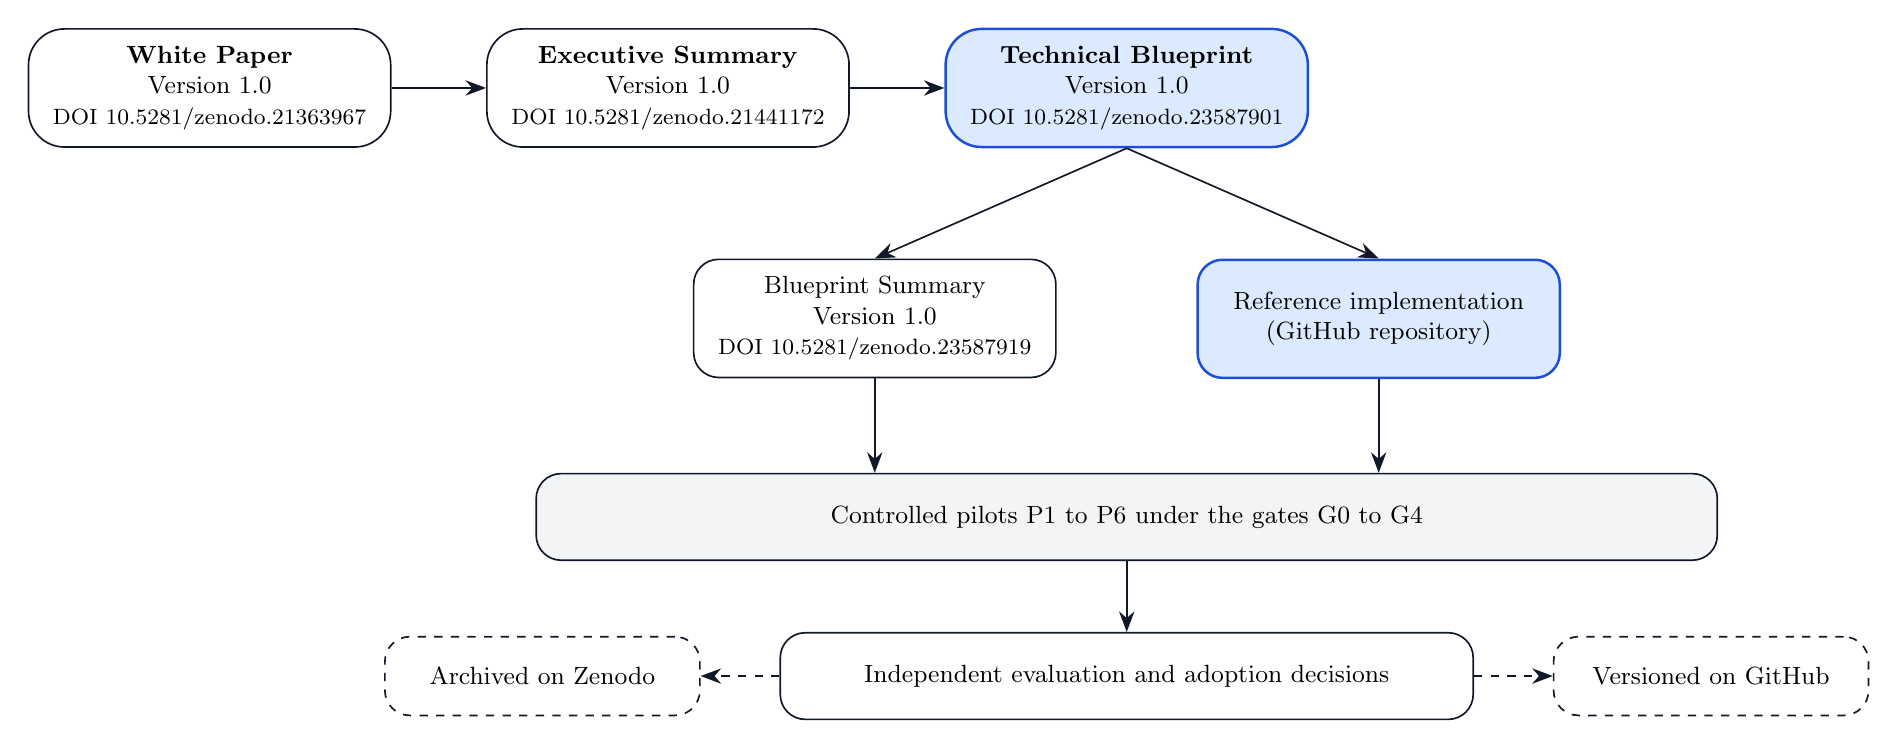
\begin{tikzpicture}[node distance=7mm and 9mm]
\node[pill, minimum width=46mm, minimum height=15mm] (wp) {\textbf{White Paper}\\Version 1.0\\{\footnotesize DOI 10.5281/zenodo.21363967}};
\node[pill, minimum width=46mm, minimum height=15mm, right=12mm of wp] (es) {\textbf{Executive Summary}\\Version 1.0\\{\footnotesize DOI 10.5281/zenodo.21441172}};
\node[key, rounded corners=13pt, minimum width=46mm, minimum height=15mm, right=12mm of es] (bp) {\textbf{Technical Blueprint}\\Version 1.0\\{\footnotesize DOI 10.5281/zenodo.23587901}};
\draw[arr] (wp) -- (es);
\draw[arr] (es) -- (bp);
\node[box, minimum width=46mm, minimum height=15mm, below=14mm of bp.south, xshift=-32mm] (sum) {Blueprint Summary\\Version 1.0\\{\footnotesize DOI 10.5281/zenodo.23587919}};
\node[key, minimum width=46mm, minimum height=15mm, below=14mm of bp.south, xshift=32mm] (code) {Reference implementation\\(GitHub repository)};
\foreach \n in {sum,code} \draw[arr] (bp.south) -- (\n.north);
\node[soft, minimum width=150mm, minimum height=11mm, below=12mm of sum, xshift=32mm] (pilots) {Controlled pilots P1 to P6 under the gates G0 to G4};
\foreach \n in {sum,code} \draw[arr] (\n.south) -- (\n.south |- pilots.north);
\node[box, minimum width=88mm, minimum height=11mm, below=9mm of pilots] (eval) {Independent evaluation and adoption decisions};
\draw[arr] (pilots) -- (eval);
\node[box, dashed, minimum width=40mm, minimum height=10mm, left=10mm of eval] (zen) {Archived on Zenodo};
\node[box, dashed, minimum width=40mm, minimum height=10mm, right=10mm of eval] (gh) {Versioned on GitHub};
\draw[darr] (eval) -- (zen);
\draw[darr] (eval) -- (gh);
\end{tikzpicture}
\end{document}
